\section{Thực nghiệm và đánh giá hai chiến lược chọn biến}

Hai chiến lược chọn biến (\texttt{ordered} và \texttt{frequency}) được chạy tự động trên cùng sáu câu đố chuẩn theo thứ tự cố định, mỗi cấu hình một lượt trên máy Windows 11, Python 3.14.6, CPU Intel Core i5-12450HX. Cột $N$ ký hiệu kích thước lưới $N\times N$.

\begin{table}[H]
\centering\footnotesize\singlespacing
\caption{Trạng thái kết thúc, quy mô KB cuối phiên và số bước suy luận}
\smallskip
\renewcommand{\arraystretch}{1.13}
\begin{tabular*}{\linewidth}{@{\extracolsep{\fill}}llrllrrrr@{}}
\toprule
\textbf{Màn} & \textbf{Chiến lược} & \textbf{N} & \textbf{Trạng thái} & \textbf{Nghiệm} & \textbf{Biến chính} & \textbf{Biến phụ} & \textbf{Mệnh đề} & \textbf{Bước} \\
\midrule
case-3x3-01 & ordered & 3 & SOLVED & UNIQUE & 9 & 156 & 491 & 7 \\
case-3x3-01 & frequency & 3 & SOLVED & UNIQUE & 9 & 156 & 491 & 7 \\
case-3x3-02 & ordered & 3 & SOLVED & UNIQUE & 9 & 144 & 455 & 7 \\
case-3x3-02 & frequency & 3 & SOLVED & UNIQUE & 9 & 144 & 455 & 7 \\
case-4x4-01 & ordered & 4 & SOLVED & UNIQUE & 16 & 364 & 1138 & 13 \\
case-4x4-01 & frequency & 4 & SOLVED & UNIQUE & 16 & 364 & 1138 & 13 \\
case-4x4-02 & ordered & 4 & SOLVED & UNIQUE & 16 & 273 & 862 & 13 \\
case-4x4-02 & frequency & 4 & SOLVED & UNIQUE & 16 & 273 & 862 & 13 \\
case-5x5-01 & ordered & 5 & SOLVED & UNIQUE & 25 & 668 & 2068 & 22 \\
case-5x5-01 & frequency & 5 & SOLVED & UNIQUE & 25 & 668 & 2068 & 22 \\
case-5x5-02 & ordered & 5 & SOLVED & UNIQUE & 25 & 654 & 2045 & 22 \\
case-5x5-02 & frequency & 5 & SOLVED & UNIQUE & 25 & 654 & 2045 & 22 \\
\bottomrule
\end{tabular*}
\end{table}

\begin{table}[H]
\centering\footnotesize\singlespacing
\caption{Chi phí tìm kiếm DPLL và thời gian chạy của từng cấu hình}
\smallskip
\renewcommand{\arraystretch}{1.13}
\begin{tabular*}{\linewidth}{@{\extracolsep{\fill}}llrrrrr@{}}
\toprule
\textbf{Màn} & \textbf{Chiến lược} & \textbf{Gọi SAT} & \textbf{Quyết định} & \textbf{Lan truyền} & \textbf{Quay lui} & \textbf{Thời gian (s)} \\
\midrule
<<<<<<< HEAD
case-3x3-01 & ordered & 34 & 48 & 2944 & 4 & 0,047 \\
case-3x3-01 & frequency & 33 & 40 & 2942 & 4 & 0,060 \\
case-3x3-02 & ordered & 30 & 34 & 2802 & 15 & 0,071 \\
case-3x3-02 & frequency & 30 & 27 & 2693 & 9 & 0,051 \\
case-4x4-01 & ordered & 84 & 518 & 29666 & 444 & 1,015 \\
case-4x4-01 & frequency & 85 & 287 & 18887 & 8 & 0,504 \\
case-4x4-02 & ordered & 93 & 168 & 12568 & 7 & 1,151 \\
case-4x4-02 & frequency & 91 & 158 & 12567 & 16 & 1,090 \\
case-5x5-01 & ordered & 162 & 193 & 43608 & 18 & 3,483 \\
case-5x5-01 & frequency & 164 & 247 & 44288 & 45 & 3,591 \\
case-5x5-02 & ordered & 182 & 752 & 55976 & 113 & 6,432 \\
case-5x5-02 & frequency & 182 & 647 & 53655 & 37 & 5,540 \\
=======
case-3x3-01 & ordered & 34 & 48 & 2944 & 4 & 0.0469 \\
case-3x3-01 & frequency & 33 & 40 & 2942 & 4 & 0.0598 \\
case-3x3-02 & ordered & 30 & 34 & 2802 & 15 & 0.0708 \\
case-3x3-02 & frequency & 30 & 27 & 2693 & 9 & 0.0511 \\
case-4x4-01 & ordered & 84 & 518 & 29666 & 444 & 1.0145 \\
case-4x4-01 & frequency & 85 & 287 & 18887 & 8 & 0.5043 \\
case-4x4-02 & ordered & 93 & 168 & 12568 & 7 & 1.1509 \\
case-4x4-02 & frequency & 91 & 158 & 12567 & 16 & 1.0898 \\
case-5x5-01 & ordered & 162 & 193 & 43608 & 18 & 3.4830 \\
case-5x5-01 & frequency & 164 & 247 & 44288 & 45 & 3.5915 \\
case-5x5-02 & ordered & 182 & 752 & 55976 & 113 & 6.4323 \\
case-5x5-02 & frequency & 182 & 647 & 53655 & 37 & 5.5400 \\
>>>>>>> e95a2af30fd2e650472e82590bb55816b145db80
\bottomrule
\end{tabular*}
\end{table}

<<<<<<< HEAD
Tổng truy vấn gồm cả tác tử đề xuất và engine kiểm chứng; thời gian bao gồm dựng KB và thực hiện vòng mở thẻ (làm tròn đến ba chữ số thập phân từ kết quả gốc tại \texttt{output/experiments/results.json}). Các phép giải ngoại tuyến để kiểm tra nghiệm duy nhất diễn ra sau khi dừng đồng hồ và được loại khỏi cả bốn bộ đếm.
=======
Số gọi SAT và các bộ đếm gộp cả truy vấn tìm bước của \texttt{LogicAgent} lẫn truy vấn xác minh trong \texttt{GameEngine.submit}. Thời gian làm tròn $10^{-4}$ giây từ \texttt{results.json}; phép kiểm tra \texttt{check\_uniqueness} chạy sau khi dừng đồng hồ nên không tính vào các bộ đếm trên.
>>>>>>> e95a2af30fd2e650472e82590bb55816b145db80

\clearpage

\subsection{So sánh hành vi phân nhánh trên cùng câu đố}

\begin{figure}[H]
\centering
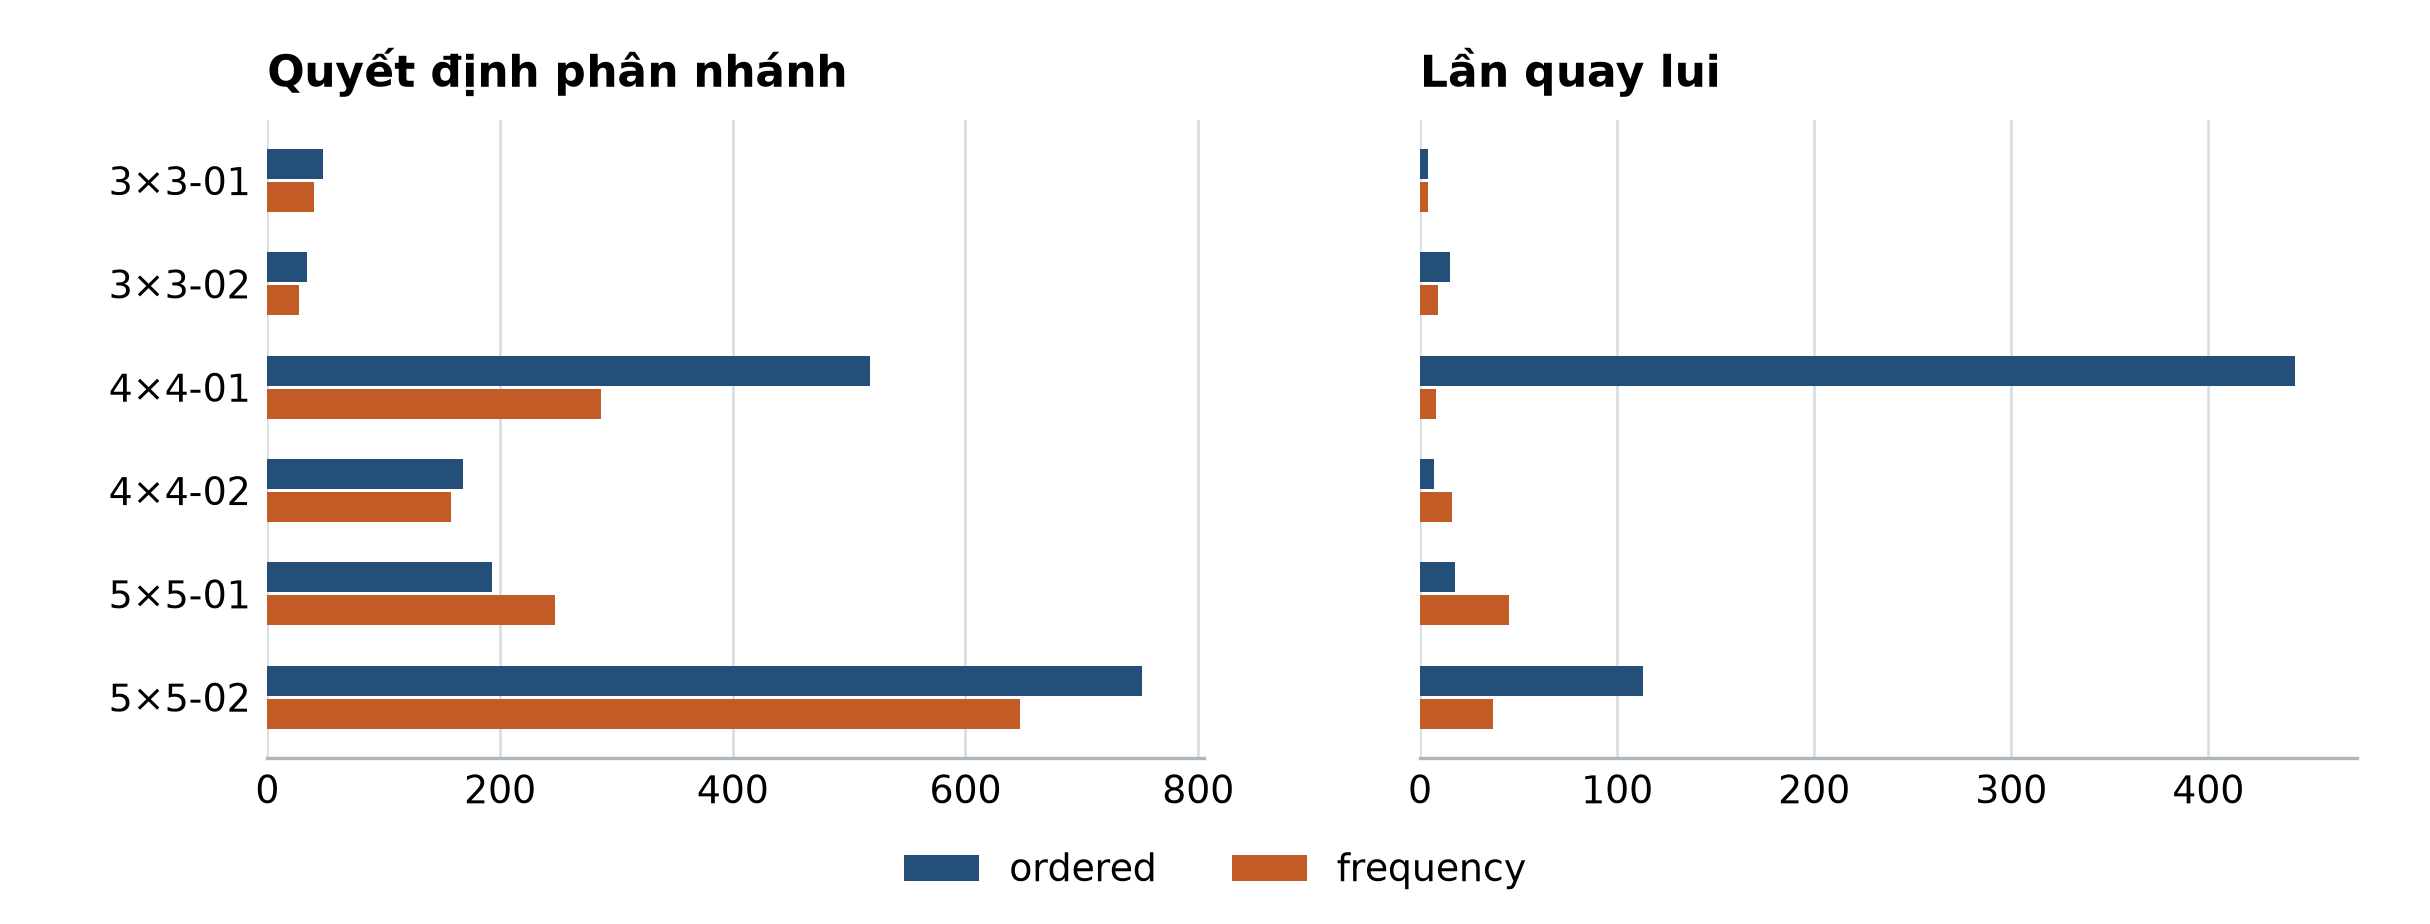
\includegraphics[width=1\linewidth]{img/chart_decisions_backtracks.png}
\caption{Số quyết định phân nhánh và số lần quay lui của hai chiến lược (hai trục ngang dùng thang riêng).}
\end{figure}

<<<<<<< HEAD
Trên màn $4\times4$-01, chuyển sang \texttt{frequency} giúp giảm từ 518 xuống 287 quyết định và từ 444 xuống 8 lần quay lui, dù số lần gọi SAT tăng nhẹ từ 84 lên 85. Trong lần giải KB ban đầu, \texttt{ordered} chọn biến số 1 (xuất hiện 4 lần trong công thức đã rút gọn), trong khi \texttt{frequency} chọn biến số 11 — một biến ô trên bàn $4\times4$ xuất hiện tới 24 lần. Gán biến liên quan đến nhiều mệnh đề có thể buộc thêm các ngưỡng đếm và làm lộ xung đột sớm.
=======
Khác biệt rõ nhất nằm ở \texttt{case-4x4-01}: chuyển sang \texttt{frequency} giảm từ 518 xuống 287 quyết định và từ 444 xuống 8 lần quay lui, dù số lần gọi SAT tăng từ 84 lên 85. Tại KB đầu tiên, \texttt{ordered} rẽ nhánh vào biến số 1 (xuất hiện 4 lần trong công thức rút gọn), còn \texttt{frequency} chọn biến số 11 (biến ô giao nhiều vùng đếm, xuất hiện 24 lần). Gán sớm biến có độ liên kết cao giúp kích hoạt lan truyền qua các ngưỡng đếm và bộc lộ xung đột nhanh hơn.
>>>>>>> e95a2af30fd2e650472e82590bb55816b145db80

Các biến phụ Tseitin cũng tham gia tính tần suất cùng biến chính. Một biến ngưỡng dùng chung ở nhiều cổng so sánh thường xuất hiện dày và tác động đồng thời lên nhiều ràng buộc. Trên màn \texttt{case-5x5-02}, với cùng 182 lần gọi SAT, \texttt{frequency} giảm từ 752 xuống 647 quyết định, hạ quay lui từ 113 xuống 37 lần và rút ngắn thời gian từ 6,4323 xuống 5,5400 giây.

Ngược lại, ở \texttt{case-5x5-01}, \texttt{ordered} chỉ cần 193 quyết định và 18 lần quay lui trong khi \texttt{frequency} tăng lên 247 và 45. Ngay ở KB mở đầu, \texttt{ordered} chọn biến số 4 và tìm được mô hình sau hai quyết định, còn \texttt{frequency} chọn biến số 18 nhưng nhánh thử \texttt{True} đầu tiên rơi vào ngõ cụt. Vì cả hai luôn thử \texttt{True} trước, ưu tiên tần suất cao vẫn có thể dẫn bộ giải vào nhánh sai trước khi quay lui.

\clearpage
\begingroup\setstretch{1.25}

\subsection{Thời gian chạy, quy mô CNF và hạn chế của hệ thống}

\begin{figure}[H]
\centering
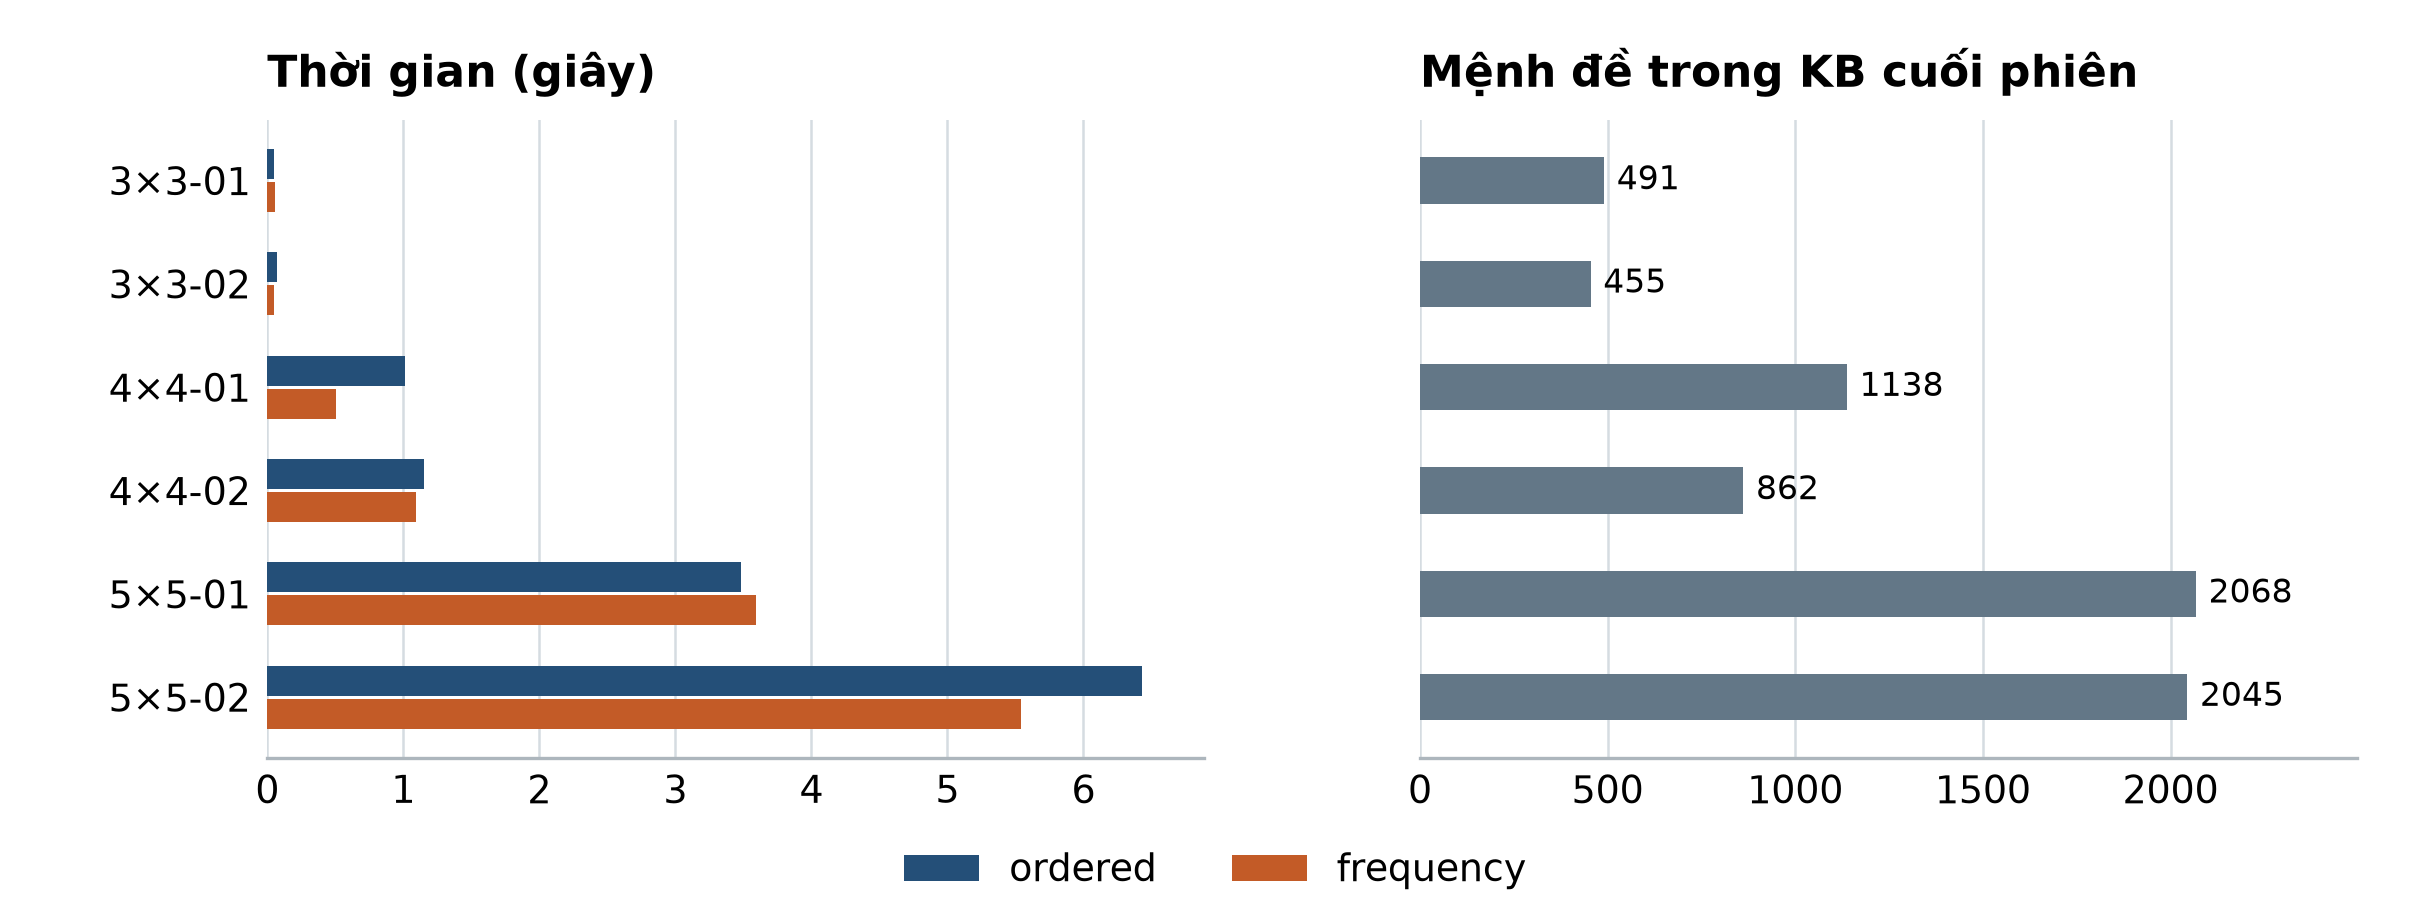
\includegraphics[width=1\linewidth]{img/chart_runtime_clauses.png}
\caption{Thời gian giải toàn màn và tổng số mệnh đề trong KB cuối phiên.}
\end{figure}

Cỡ bàn không quyết định toàn bộ chi phí giải. Hai màn $5\times5$ cùng mở 22 thẻ và có số mệnh đề cuối gần nhau (2\,068 và 2\,045), nhưng \texttt{case-5x5-02} phân nhánh nhiều hơn nên mất 5,54--6,43 giây so với 3,48--3,59 giây của \texttt{case-5x5-01}. Ở \texttt{case-4x4-01}, việc giảm mạnh quay lui giúp \texttt{frequency} rút nửa thời gian (1,0145 xuống 0,5043 giây), còn trên bàn $3\times3$ thời gian dưới 0,08 giây nên chịu ảnh hưởng đáng kể bởi chi phí đếm tần suất và tải hệ thống.

Khi hai chiến lược trả về mô hình cơ sở khác nhau, tập giá trị \texttt{True}/\texttt{False} ghi nhận sẵn cho các biến chính cũng thay đổi, làm số lần gọi SAT đôi khi lệch 1--2 truy vấn dù mở cùng số thẻ. Tại \texttt{case-4x4-02}, \texttt{frequency} giảm quyết định (158 so với 168) nhưng quay lui nhiều hơn (16 so với 7), cho thấy cần đánh giá kết hợp nhiều chỉ số.

Cả 12 lượt đều đạt \texttt{SOLVED} và kiểm tra ngoại tuyến đạt \texttt{UNIQUE}. Nếu gặp màn thiếu dữ kiện hoặc mâu thuẫn, vòng lặp ghi nhận nguyên trạng thái \texttt{UNKNOWN}, \texttt{INCONSISTENT} hoặc \texttt{TIMEOUT} vào bảng kết quả. Hạn mặc định mỗi màn là 30 giây, kiểm tra giữa các bước kèm hạn riêng trên từng truy vấn SAT.

Về hạn chế, DPLL thuần Python hiện quét lại danh sách mệnh đề ở mỗi bước lan truyền và rút gọn, chưa cài đặt kỹ thuật hai literal canh (\emph{two-watched literals}) hay học mệnh đề xung đột như CDCL. Ngoài ra, bộ thực nghiệm mới đo một lượt mỗi cấu hình trên sáu màn nên phù hợp để phân tích hành vi tìm kiếm cụ thể hơn là ước lượng phân bố thống kê trên lưới lớn hơn.

\par\endgroup
